\documentclass{article}

\usepackage[french]{babel}
\usepackage[utf8]{inputenc}
\usepackage{amsmath}
\usepackage{graphicx}
\usepackage{float}

\graphicspath{{img/}}

%%%%%%%%%%%%%%%% Lengths %%%%%%%%%%%%%%%%
\setlength{\textwidth}{15.5cm}
\setlength{\evensidemargin}{0.5cm}
\setlength{\oddsidemargin}{0.5cm}

%%%%%%%%%%%%%%%% Variables %%%%%%%%%%%%%%%%
\def\projet{3}
\def\titre{Compression d'image à travers la factorisation SVD}
\def\groupe{2}
\def\equipe{3}
\def\responsible{tpitault}
\def\secretary{jmeurgues}
\def\others{matguedon, alamhamdi001, aliard}

\begin{document}

%%%%%%%%%%%%%%%% Header %%%%%%%%%%%%%%%%
\noindent\begin{minipage}{0.98\textwidth}
  \vskip 0mm
  \noindent
  { \begin{tabular}{p{7.5cm}}
      {\bfseries \sffamily
        Projet \projet} \\ 
      {\itshape \titre}
    \end{tabular}}
  \hfill 
  \fbox{\begin{tabular}{l}
      {~\hfill \bfseries \sffamily Groupe \groupe\ - Equipe \equipe
        \hfill~} \\[2mm] 
      Responsable : \responsible \\
      Secrétaire : \secretary \\
      Codeurs : \others
    \end{tabular}}
  \vskip 4mm ~

  ~~~\parbox{0.95\textwidth}{\small \textit{Résumé~:} \sffamily Ce projet consiste à programmer un algorithme permettant de faire de la compression d'images en utilisant des techniques matricielles basées sur la factorisation SVD. La première partie met en place les fonctions utilitaires pour manipuler les matrices de Householder. La deuxième et la troisième partie consistent à transformer une matrice en une matrice bidiagonale puis en une matrice diagonale. La dernière partie applique ces transformations à l'algorithme de compression d'image par transformation SVD.  }
  \vskip 1mm ~
\end{minipage}

%%%%%%%%%%%%%%%% Main part %%%%%%%%%%%%%%%%
\section*{Introduction}

Ce projet a pour but de créer un algorithme qui permet de compresser des images. Pour ce faire, nous devrons réaliser une décomposition en valeurs singulières (SVD) d'une matrice $A$ quelconque. C'est-à-dire que l'on cherche à la mettre sous la forme :
\begin{equation}
    \displaystyle{ A = U \times S \times V }
\end{equation}
avec $U$ et $V$ des matrices orthogonales de dimensions respectives $m \times k$ et $k \times n$ où $k = min(m,n)$, et $S$ une matrice de dimensions $k \times k$ diagonales réelle; ses éléments diagonaux sont positifs et forment une suite décroissante.
\section{Transformations de Householder}

Pour commencer, nous cherchons à manipuler les matrices de Householder. Une telle matrice s'écrit sous la forme :
\begin{equation}
    \displaystyle{H = Id - 2 \times U.^tU}
\end{equation}
avec $Id$ la matrice identité de taille $n$ et $U$ un vecteur de taille $n$ et de norme euclidienne 1.

\paragraph{}
En premier lieu, nous réalisons un algorithme permettant de choisir un $U$ pour chaque couple de vecteur $X$ et $Y$ tel que $H.X = Y$. Il s'écrit sous la forme
\begin{equation}
    U=\frac{X-Y}{||X-Y||}
\end{equation}
Ainsi, nous pouvons donc retrouver la matrice de Householder qui renvoie $X$ sur $Y$.

\paragraph{}
Nous avons ensuite réalisé une fonction qui calcule le produit entre une matrice de Householder et un vecteur, puis entre une matrice de Householder et une autre matrice (comme ensemble de vecteurs). En exploitant le produit scalaire, nous avons pu atteindre une complexité linéaire.
En utilisant la définition de la matrice de Householder, nous avons: 
\begin{equation}
    \displaystyle{H.v = v - 2 \times U.^tU.v}
\end{equation}

\paragraph{}
L'algorithme calculant le produit entre une matrice de Householder et un vecteur prend en paramètres le vecteur $U$ qui définit la matrice de Householder et un vecteur $v$. Il utilise une fonction qui calcule, en temps linéaire, le produit scalaire des deux vecteurs $^{t}U$ et $v$.

\paragraph{}
Ensuite, pour optimiser le produit matriciel entre une matrice de Householder et une autre matrice, afin d'éviter de faire un produit matrice-matrice, nous avons opté pour le produit matrice-vecteur utilisé précédemment. L'algorithme de produit matriciel prend en paramètre le vecteur $U$ de la matrice de Householder et une matrice $M$ et renvoie le produit en temps quadratique $O(n^2)$. \\[0.2cm]
En comparaison, le produit matriciel classique a une complexité cubique $O(n^3)$, ce qui est moins optimisé que notre fonction.
 
\section{Mise sous forme bidiagonale}

La décomposition SVD nécessite de mettre la matrice sous une forme bidiagonale. Pour cela, nous avons appliqué un algorithme utilisant les matrices de Householder déterminées dans la partie 1. L'idée est d'obtenir une matrice $BD$ bidiagonale telle que $A = QR \times BD \times QL$ avec $QR$ et $QL$ les matrices, de changement de base, gauche et droite. \\
Pour illustrer le principe de l'algorithme, nous utiliserons la matrice en Figure \ref{fig:matrice_ex}.
\begin{itemize}
    \item Initialement, on a $BD = A$ et les deux matrices $QR$ et $QL$ sont des matrices identités. 
    \item Dans un premier temps, on extrait le vecteur colonne $C1$ et on calcule la matrice de Householder l'envoyant sur un vecteur de même norme, mais ne possédant qu'un coefficient non nul.
    \item Ensuite, on remplace la colonne de la matrice $BD$ par le vecteur utilisé pour créer la matrice de Householder puis on multiplie cette matrice à la matrice de changement de base pour que cette dernière soit en accord avec la nouvelle matrice $BD$.
    \item Dans un second temps, on répète l'opération sur la ligne L1 puis on modifie $BD$ et $QR$ sur le même principe que précédemment. 
    \item Enfin, on répète cette opération sur toutes les colonnes et lignes de la matrice en Figure \ref{fig:matrice_ex}.
\end{itemize}
\paragraph{}
L'idée de l'algorithme est donc de ne garder que les coefficients $a_1, a_2, ..., a_n$ et $b_1, b_2, ..., b_n$ non nuls dans les colonnes et les lignes. La matrice $BD$ devient donc bidiagonale.
On peut noter qu'à chaque itération de l'algorithme, il existe un invariant de boucle : $$A = QR\times BD\times QL$$

\begin{figure}[H]
    \centering
    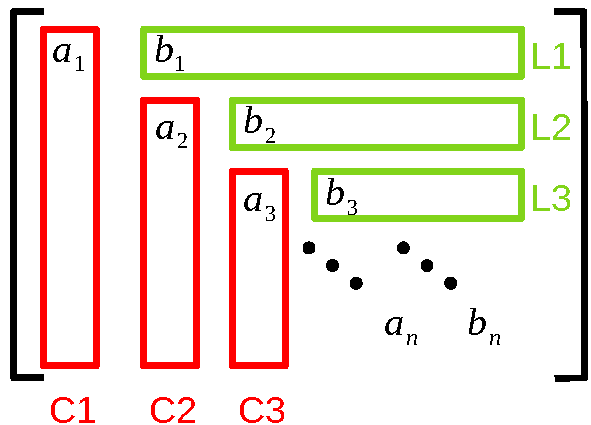
\includegraphics[scale=0.5]{matrice_exemple.pdf}
    \caption{Matrice illustrant le principe de fonctionnement de l'algorithme de bidiagonalisation}
    \label{fig:matrice_ex}
\end{figure}

\section{Transformations QR}

Pour effectuer la décomposition SVD, une fois la mise sous forme bidiagonale effectuée, il faut appliquer la transformation QR un certain nombre de fois à la matrice bidiagonale.

\paragraph{}
Nous avons testé l'algorithme permettant de réaliser la décomposition SVD, en vérifiant que, tout au long du programme, $U \times S \times V$ est une matrice bidiagonale, ce qui garantit la correction de notre algorithme. 

\paragraph{}
Puis nous avons tracé un graphe qui illustre la convergence de la matrice $S$ vers une matrice diagonale. Ce graphe, visible en Figure \ref{fig:facto_QR}, montre la norme de l'extra-diagonale en fonction du nombre d'itérations de la factorisation QR. Nous pouvons observer que l'on converge rapidement vers une matrice diagonale.

\begin{figure}[H]
    \centering
    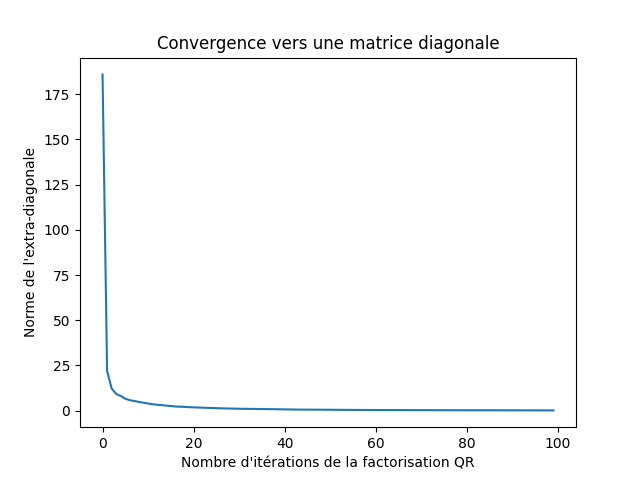
\includegraphics[scale=0.7]{convergence_facto_QR.png}
    \caption{Convergence de S vers une matrice diagonale selon le nombre de factorisation QR effectuées}
    \label{fig:facto_QR}
\end{figure}

\paragraph{}
Nous avons également montré que, tout au long du programme, nous avions bien l'invariant suivant vérifié : "$S$, $R1$ et $R2$ sont toujours bidiagonales".
En effet, à l'entrée du programme, la matrice $S$ est déjà bidiagonale supérieure.
Ainsi, $^tS$ est bidiagonale inférieure.
Comme l'algorithme QR préserve la forme de la matrice tridiagonale à chaque étape, alors R1 est une matrice tridiagonale. De plus, comme $R1$ est aussi triangulaire supérieure, on en déduit que R1 est bidiagonale supérieure. On suit le même raisonnement pour prouver que R2 est aussi bidiagonale supérieure.

\paragraph{}
Nous avons ensuite simplifié l'algorithme pour qu'il soit plus rapide. Notre premier algorithme faisait deux fois appel à la fonction \verb|linalg.qr| de \verb|numpy| et à la fonction \verb|dot|. Le nouvel algorithme ne fait qu'un simple appel à ces fonctions. On a donc réduit la complexité de la fonction de transformation QR.

\paragraph{}
Enfin, la décomposition SVD demande à ce que les éléments de la matrice $S$ soient positifs, ordonnés de manière décroissante. L'algorithme correspondant prend en paramètre les deux matrices $U$ et $S$ et les modifie de sorte que $S$ vérifie la propriété citée précédemment et que la multiplication $U\times S$ soit inchangée pour que $U\times S\times V$ soit bidiagonale. Afin de trier la diagonale en fonction de la valeur absolue de ses éléments, on effectue l'opération suivante:
\begin{center}
    \[\begin{pmatrix}
        u_{1,1} & u_{1,2} & \cdots & u_{1,n} \\
        u_{2,1} & u_{2,2} & \cdots & u_{2,n} \\
        \vdots & \vdots & \ddots & \vdots \\
        u_{n,1} & u_{n,2} & \cdots & u_{n,n}
    \end{pmatrix}
    \begin{pmatrix}
        s_{1,1} & 0 & \cdots & 0 \\
        0 & s_{2,2} & \cdots & 0 \\
        \vdots & \vdots & \ddots & \vdots \\
        0 & 0 & \cdots & s{n,n}
    \end{pmatrix}\]\\
\end{center}

\begin{equation}
    i\ieme{} colonne de U \gets i\ieme{} colonne de U \times \frac{OldDiagonaleS[i]}{NewDiagonaleS[i]}
\end{equation}
où \texttt{OldDiagonaleS} est la liste des éléments de l'ancienne diagonale de S et \texttt{NewDiagonaleS} est la nouvelle liste triée des éléments de la diagonale de S et positifs. Dans le cas où l'élément de la diagonale de S est négatif, on multiplie la colonne lui correspondant dans la matrice U par -1.



\section{Application à la compression d'image}

Pour compresser une image stockée sous la forme d'une matrice carrée $A$, il s'agit de la mettre sous la forme $A = U \times S \times V$ grâce à la factorisation SVD, puis de s'intéresser aux valeurs de la diagonale de $S$. En effet, on appelle compression au rang $k$ le fait d'annuler les termes diagonaux de $S$ strictement supérieurs à $k$. Ainsi, on peut stocker la matrice $S$ dans une liste de taille $k$ correspondant aux termes diagonaux non nul après la compression.

\paragraph{}
Pour réaliser la compression au rang k d'une image, notre algorithme crée une matrice pour chaque couleur r, g, b de l'image et reprend les étapes suivantes pour chacune d'elles :
\begin{itemize}
    \item (L, BD, R) $\leftarrow$ bidiagonalisation(matrice)
    \item (U, S, V) $\leftarrow$ transformation\_QR(BD, 100) 
    \item (U, S) $\leftarrow$ termes de la diagonale de $S$ positifs et décroissants
    \item Annulation des valeurs des rangs supérieurs à k
    \item Reconstruction de $A$ : $L \times U \times S \times V \times R$
\end{itemize}
\paragraph{}
Bien que l'on retrouve l'image originale dans celle compressée, nous avons observé plusieurs problèmes. Tout d'abord, il y a des dégradations sur les bords haut et gauche de l'image compressée. Ensuite, certaines valeurs de la matrice étaient négatives ou supérieures à 1. Or, la matrice image ne peut contenir que des valeurs entre 0 et 1. Pour visualiser à quels pixels correspondent ces valeurs, nous avons choisi de mettre en rouge les pixels ayant une valeur négative et en vert ceux ayant une valeur supérieure à 1. En Figure \ref{fig:compression-img}, on peut observer le résultat de ces modifications. On remarque que pour les pixels blancs, c'est-à-dire les pixels ayant des valeurs proches de 1, ces dépassements sont sûrement dû aux imprécisions du système. En revanche, nous n'avons pas réussi à déterminer la cause exacte de la présence des pixels rouges, mais cela est très probablement en lien avec la fonction de bidiagonalisation qui renvoie des valeurs extrêmements imprécises. 

\paragraph{}
Par ailleurs, nous n'avons pas réussi à gagner de la place à l'aide de la compression. En effet, au lieu d'avoir la matrice $A$ de taille $n \times m$ stockée en mémoire, on aura $U$, $S$ et $V$ de tailles respectives $n^2$, $n \times m$ et $m^2$. Une fois $S$ compressée au rang $k$, on peut la stocker comme un tableau de taille $k$. En revanche, nous n'avons pas trouvé comment stocker les matrices orthogonales $U$ et $V$ de manière à gagner de la place par rapport à $A$.

\begin{figure}[H]
   \begin{minipage}{0.5\textwidth}
        \centering
        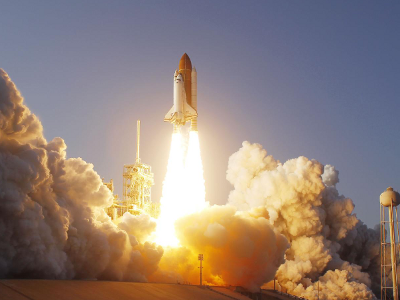
\includegraphics[width=0.9\linewidth]{original.png} \\
        Original
    \end{minipage}\hfill
   \begin{minipage}{0.5\textwidth}
        \centering
        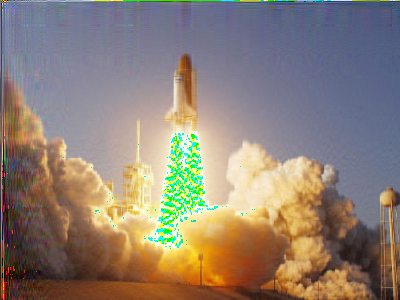
\includegraphics[width=0.9\linewidth]{compression_rang_50.png} \\
        Rang 50
   \end{minipage}\hfill
   \caption{Compression sur différents rangs}
   \label{fig:compression-img}
\end{figure}

\section{Conclusion}
Nous avons une solution algorithmique qui s'approche de ce qui était attendu. Néanmoins, l'image obtenue est déformée et notre algorithme de bidiagonalisation ne fonctionne pas correctement. De plus, il nous manque un moyen astucieux de stocker $U$ et $V$ afin d'avoir un vrai gain de place pour le stockage de l'image.

\end{document}
